\documentclass[11pt,a4paper]{article}
\usepackage[margin=2.2cm]{geometry}
\usepackage{graphicx}
\usepackage{booktabs}
\usepackage{caption}
\usepackage{subcaption}
\usepackage{float}
\usepackage{amsmath}
\usepackage{xcolor}
\usepackage{multirow}
\usepackage[hidelinks]{hyperref}
\usepackage{enumitem}
\graphicspath{{../plots/}}
\setlength{\parskip}{4pt}
\captionsetup{font=small,labelfont=bf}

% ------------------------------------------------------------------
% TEAM
% ------------------------------------------------------------------
\newcommand{\teamtable}{%
\begin{tabular}{ll}
\toprule
Name & Roll number \\
\midrule
Pranav & 24B1074 \\
Atharva & 24B0996 \\
Divyaansh & 24B0981 \\
Sufiyan & 24B0935 \\
\bottomrule
\end{tabular}}

\title{\textbf{CS683 PA1, Task 2: Matrix Multiplication for Inference}\\[4pt]
\large Software prefetching, SIMD, their combination, and a run inside llama.cpp}
\author{\teamtable}
\date{Autumn 2026}

\begin{document}
\maketitle

\section{Setup and methodology}

\paragraph{Machine.} Intel Core i7-13700HX (Raptor Lake). Every run was pinned to CPU~0, a P-core, with \texttt{taskset}, governor \texttt{performance}. L1-D 48\,KB 12-way, L2 1.25\,MB per P-core, L3 30\,MB, 64\,B lines. This part has no AVX-512, so the SIMD widths we could study are 128-bit (SSE) and 256-bit (AVX2 with FMA). We toggled the hardware prefetchers through MSR \texttt{0x1a4}: \texttt{wrmsr -a 0x1a4 0xf} disables the L2 streamer, the L2 adjacent-line prefetcher, the L1 streamer and the L1 IP prefetcher, and \texttt{0x0} turns them back on. We re-enabled them after every experiment.

\paragraph{Build and harness.} Pinned flags \texttt{-std=c++17 -O2 -fno-tree-vectorize -mavx2 -mfma}, unchanged. The harness takes the median of 3 timed repetitions after one warm-up, checks every stage against \texttt{matmul\_naive} (relative tolerance $10^{-4}$), and reports speedup as $t_{\text{naive}}/t_{\text{stage}}$ on the same input. The prefetch parameters (distance \texttt{PF\_D} in floats, hint \texttt{PF\_L}, panel width \texttt{JC}) are compile-time macros, so a sweep recompiles rather than editing the source. Counters come from \texttt{perf stat} on the P-core PMU: \texttt{L1-dcache-load-misses}, \texttt{l2\_rqsts.miss}, \texttt{LLC-load-misses}, \texttt{instructions}, and the three \texttt{sw\_prefetch\_access.\{t0, t1\_t2, nta\}} events that count issued software prefetches by hint. We measured instruction counts with an isolated single-call driver, because the harness's naive reference and warm-ups would otherwise swamp the count.

\paragraph{Layout.} $C[i][j] = \sum_p A[i][p]\,B[j][p]$ with $A$ ($M\times K$), $B$ ($N\times K$, stored transposed) and leading dimensions \texttt{lda, ldb, ldc}. This is ggml's \texttt{mul\_mat} form. The contraction index is contiguous in both operands, so the inner loop is a unit-stride dot product.

\paragraph{Kernels.} Four kernels appear in this report.

\texttt{matmul\_simd} (Task 2B, graded) is a $1\times4$ register-tiled AVX2 micro-kernel. One 8-float vector of row $A_i$ is loaded and reused against 4 rows of $B$ with 4 independent \texttt{\_mm256\_fmadd\_ps} accumulators; a horizontal sum runs once per output; scalar tails handle $K \bmod 8$ and $N \bmod 4$. There is no cache blocking.

The scalar prefetch-only kernel (Task 2A, ungraded file \texttt{matmul\_prefetch\_scalar.cpp}) is the naive triple loop with one \texttt{\_mm\_prefetch(b+p+D, hint)} added in the inner loop. Its only purpose is to isolate software prefetching from every other technique, which is how the assignment document defines Task 2A.

\texttt{matmul\_prefetch} (Task 2A/2C stage, graded) is the $1\times4$ SIMD micro-kernel with the $j$ loop blocked into panels of \texttt{JC}=64 rows of $B$, so a $64\times K$ panel stays in L2 and is reused across all $M$ rows of $A$, plus \texttt{\_mm\_prefetch} on the four $B$ streams \texttt{PF\_D} floats ahead. Building with \texttt{PF\_D}=0 compiles the prefetches out and gives the pure-tiling baseline for the with/without comparison.

\texttt{matmul\_optimized} (Task 2C, graded, and the kernel injected into llama.cpp) uses a $4\times4$ register block with 16 \texttt{\_\_m256} accumulators. Each $A$ vector feeds 4 FMAs and each $B$ vector feeds 4, which doubles the arithmetic intensity of the $1\times4$ kernel. It uses \texttt{JC}=32 panels (the best of a 16 to 96 sweep), unrolled accumulation, vectorised tails for ragged $M$, $N$, $K$, and optional \texttt{\_mm\_prefetch} under the same macros. A full SSE port of this kernel (\texttt{matmul\_optimized128.cpp}, ungraded) served for the width study.

All kernels pass the harness on $256^3$ and $1024^3$ and on the ragged shapes $37\times53\times71$, $1\times129\times130$, $255\times257\times129$, $5\times3\times2$ and $3\times3\times3$.

\section{Task 2A: software prefetching}

\subsection{Prefetching in isolation: the scalar kernel}

\begin{table}[H]
\centering\small
\caption{Scalar prefetch-only kernel. Speedup as defined in the assignment, $t_{\text{without}}/t_{\text{with}}$, distance 64 floats, hint T0. Data: \texttt{task2a\_scalar\_prefetch.txt}.}
\begin{tabular}{lrrrrr}
\toprule
$M=N=K$ & 128 & 256 & 512 & 1024 & 2048 \\
\midrule
without SW prefetch (ms) & 0.666 & 6.06 & 54.5 & 436.1 & 3628.9 \\
with SW prefetch (ms)    & 1.113 & 12.18 & 102.2 & 857.1 & 7113.1 \\
speedup                  & 0.60$\times$ & 0.50$\times$ & 0.53$\times$ & 0.51$\times$ & 0.51$\times$ \\
\bottomrule
\end{tabular}
\end{table}

Adding one prefetch instruction to the scalar loop halves throughput at every size. The distance sweep at $N=1024$ (8, 16, 32, 64, 128, 256 floats) sits at 0.51 to 0.52$\times$ throughout, and the hint sweep (T0, T1, T2, NTA) is just as flat at 0.51 to 0.52$\times$. The \texttt{sw\_prefetch\_access} counters say why. The scalar loop issues one prefetch per element, $5.37\times10^9$ of them for a $1024^3$ product, which is 16 redundant prefetches for every 64-byte line. The inner loop is one load, one multiply-add and one prefetch, so the prefetch doubles the dynamic instruction count of a loop that was already issue-bound, and no distance or hint can buy that back. The prefetches do still work at the cache level. L1-D misses fall by 42 to 45\% at every size (40.3\,M to 22.6\,M at 1024, 235.8\,M to 140.7\,M at 2048), while L2 and LLC misses stay the same. Turning the hardware prefetchers off changes nothing (0.52$\times$ with HW off, 0.53$\times$ with HW on), because the cost here is the overhead rather than latency. The vector kernels avoid this by issuing one prefetch per 8-float step.

\subsection{Prefetching on the blocked SIMD kernel (\texttt{matmul\_prefetch})}

\begin{table}[H]
\centering\small
\caption{\texttt{matmul\_prefetch}: speedup over naive with prefetch on (distance 64, T0), and the assignment-defined speedup $t_{\text{without}}/t_{\text{with}}$. Data: \texttt{task2a\_sweep.txt}, \texttt{task2a\_swpf\_vs\_size.txt}.}
\label{tab:2a-size}
\begin{tabular}{lrrrrrr}
\toprule
$M=N=K$ & 128 & 256 & 512 & 1024 & 1536 & 2048 \\
\midrule
speedup over naive (SW pf on)  & 13.2$\times$ & 11.7$\times$ & 14.1$\times$ & 12.5$\times$ & 12.6$\times$ & 12.1$\times$ \\
GFLOP/s (SW pf on)             & 70.1 & 65.9 & 66.0 & 60.8 & 61.2 & 57.8 \\
without SW pf (ms)             & 0.046 & 0.420 & 3.456 & 28.70 & 103.4 & 246.2 \\
with SW pf (ms)                & 0.067 & 0.509 & 3.910 & 34.64 & 111.8 & 280.7 \\
$t_{\text{without}}/t_{\text{with}}$ & 0.69$\times$ & 0.83$\times$ & 0.88$\times$ & 0.83$\times$ & 0.93$\times$ & 0.88$\times$ \\
\bottomrule
\end{tabular}
\end{table}

\begin{figure}[H]
\centering
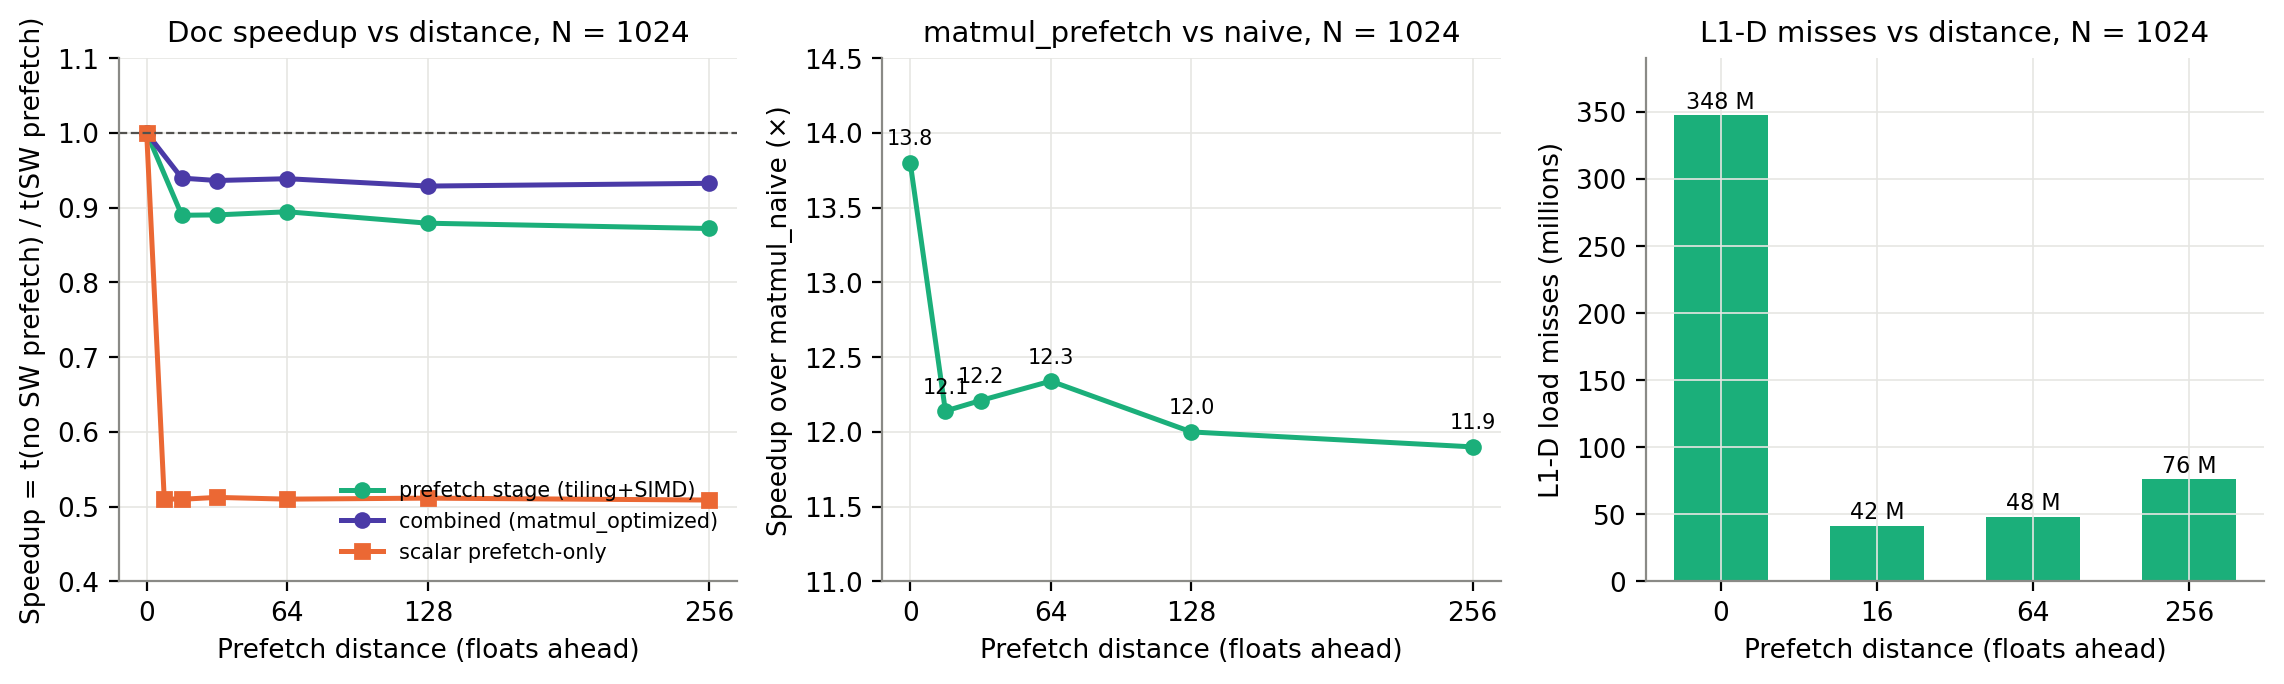
\includegraphics[width=\textwidth]{task2_prefetch_degree.png}
\caption{Prefetch distance. Left: assignment-defined speedup versus distance for the three prefetching kernels at $N=1024$. Middle: \texttt{matmul\_prefetch} speedup over naive versus distance. Right: its L1-D load misses versus distance (\texttt{task2a\_cachemiss\_params.txt}).}
\label{fig:degree}
\end{figure}

\begin{figure}[H]
\centering
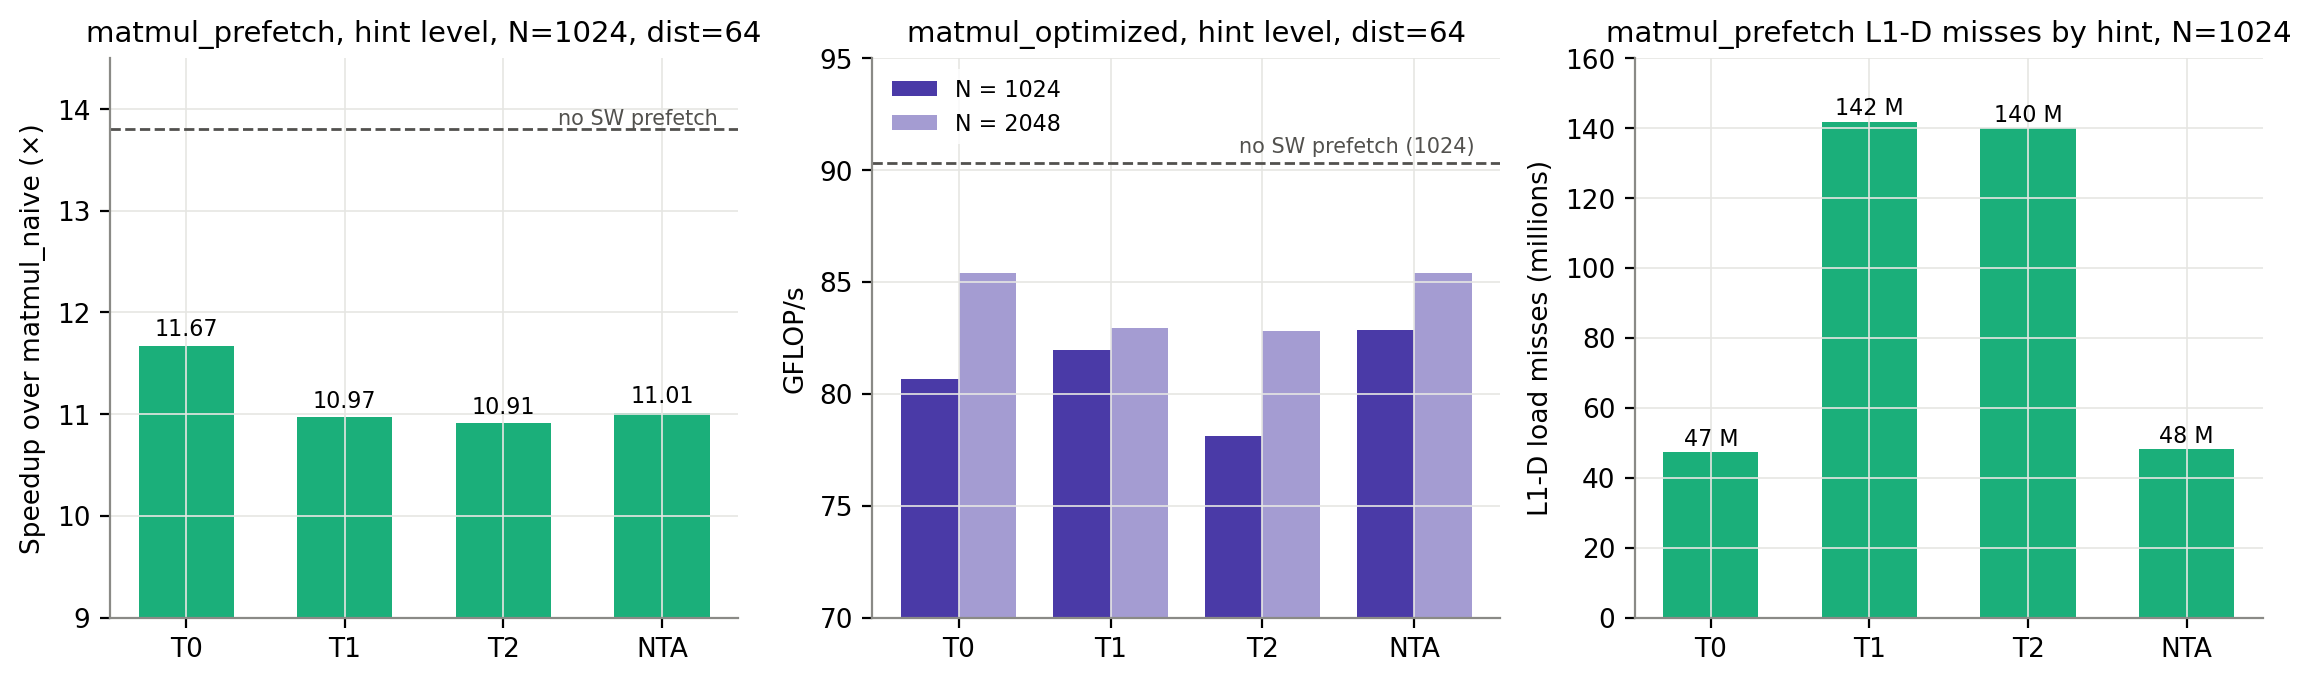
\includegraphics[width=\textwidth]{task2_prefetch_level.png}
\caption{Cache fill level. Left: \texttt{matmul\_prefetch} at distance 64 for the four hints, dashed line is the no-prefetch build. Middle: the combined kernel at $N=1024$ and $2048$. Right: L1-D misses of \texttt{matmul\_prefetch} by hint.}
\label{fig:level}
\end{figure}

\begin{table}[H]
\centering\small
\caption{\texttt{matmul\_prefetch}, $N=1024$: cache misses versus prefetch distance and hint (\texttt{task2a\_cachemiss\_params.txt}) and issued software prefetches (\texttt{task2a\_swpf\_counters.txt}).}
\label{tab:2a-params}
\begin{tabular}{l rrr r}
\toprule
setting & L1-D misses & L2 misses & LLC misses & \texttt{sw\_prefetch\_access} (t0 / t1\_t2 / nta) \\
\midrule
no SW prefetch          & 347.8\,M & 418.1\,M & 23.5\,K & 11\,K / 0 / 0 \\
dist 16, T0             & 41.6\,M  & 418.1\,M & 16.2\,K & 671\,M / 0 / 0 \\
dist 64, T0             & 48.3\,M  & 418.1\,M & 15.6\,K & 671\,M / 0 / 0 \\
dist 256, T0            & 76.5\,M  & 418.2\,M & 32.2\,K & 671\,M / 0 / 0 \\
dist 64, T1             & 141.8\,M & 417.9\,M & 18.0\,K & 12\,K / 671\,M / 0 \\
dist 64, T2             & 139.9\,M & 418.2\,M & 18.7\,K & 12\,K / 671\,M / 0 \\
dist 64, NTA            & 48.2\,M  & 420.7\,M & 18.6\,K & 12\,K / 0 / 671\,M \\
\bottomrule
\end{tabular}
\end{table}

\begin{table}[H]
\centering\small
\caption{\texttt{matmul\_prefetch}: cache misses versus matrix size, without and with software prefetch (distance 64, T0). Data: \texttt{task2a\_cachemiss\_vs\_size.txt}.}
\label{tab:2a-miss-size}
\begin{tabular}{l rr rr rr}
\toprule
& \multicolumn{2}{c}{L1-D misses} & \multicolumn{2}{c}{L2 misses} & \multicolumn{2}{c}{LLC misses} \\
\cmidrule(lr){2-3}\cmidrule(lr){4-5}\cmidrule(lr){6-7}
$N$ & without & with & without & with & without & with \\
\midrule
256  & 4.75\,M & 1.04\,M & 163\,K & 165\,K & 3.6\,K & 3.6\,K \\
1024 & 348.2\,M & 48.4\,M & 418.3\,M & 418.2\,M & 25.7\,K & 16.3\,K \\
2048 & 2765\,M & 390\,M & 3363\,M & 3385\,M & 2.35\,M & 1.07\,M \\
\bottomrule
\end{tabular}
\end{table}

\begin{figure}[H]
\centering
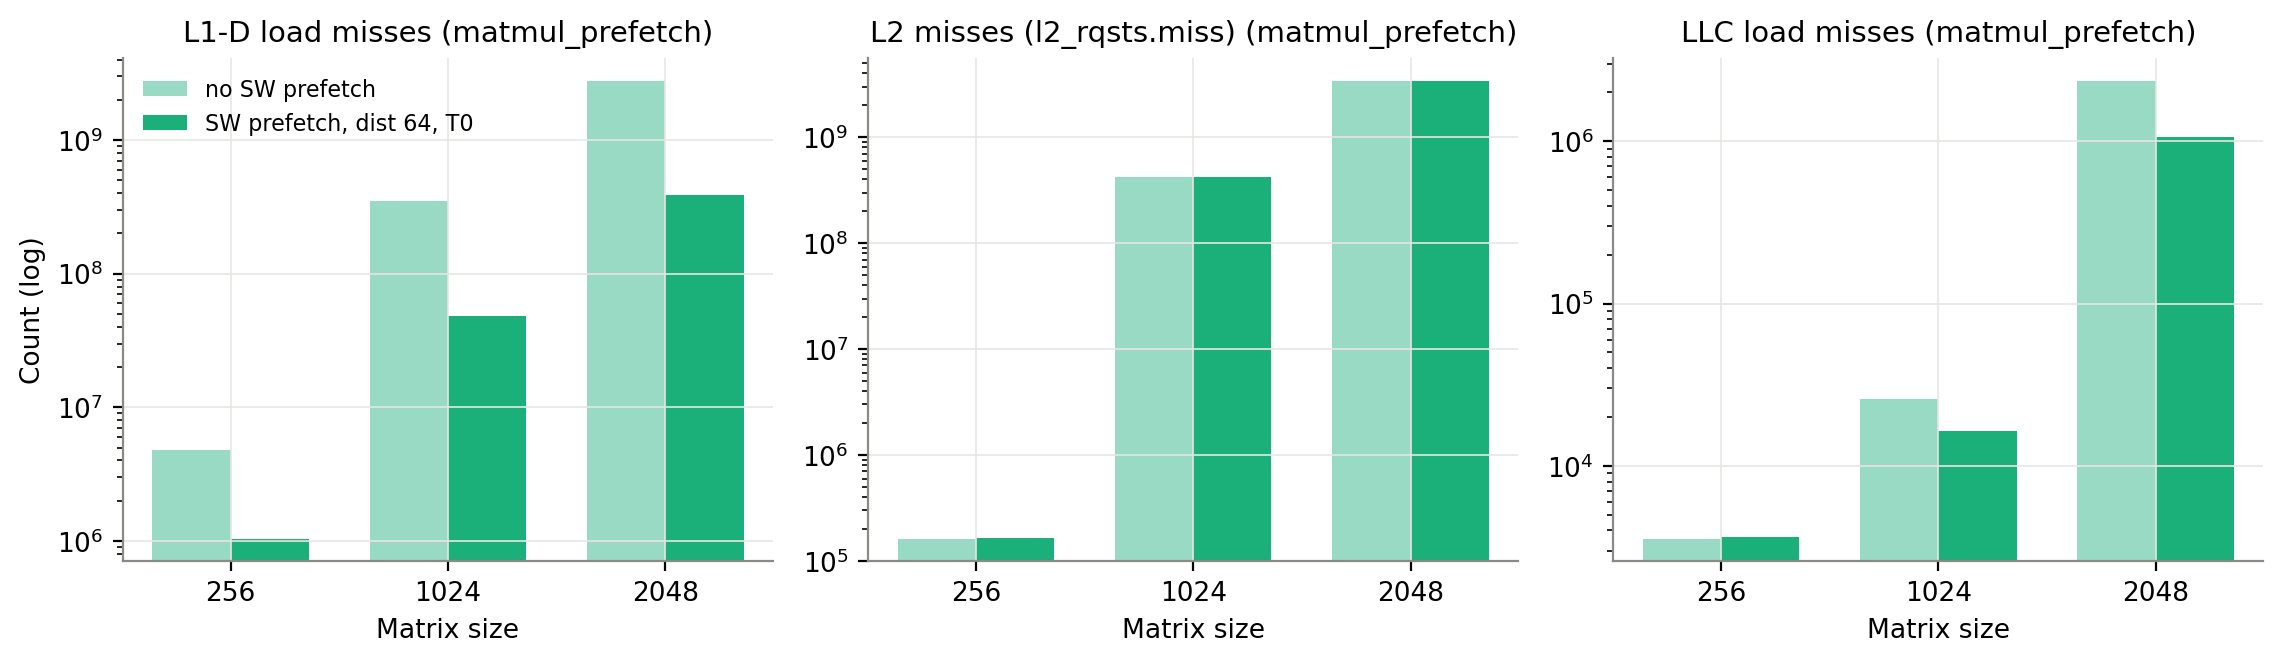
\includegraphics[width=\textwidth]{task2_cachemiss.png}
\caption{Cache misses at each level versus size for \texttt{matmul\_prefetch}, with and without software prefetch (log scale).}
\end{figure}

\subsection{Effect of the hardware prefetchers}

\begin{table}[H]
\centering\small
\caption{Hardware prefetchers enabled/disabled (MSR \texttt{0x1a4}), $N=1024$, software prefetch at distance 64/T0 or compiled out. \texttt{task2a\_hwpf.txt}, \texttt{task2a\_scalar\_hwpf.txt}, \texttt{task2c\_hwpf.txt}.}
\label{tab:hwpf}
\begin{tabular}{l l rr}
\toprule
kernel & HW prefetchers & SW prefetch off & SW prefetch on \\
\midrule
scalar prefetch-only (speedup vs naive) & off & 1.00$\times$ & 0.52$\times$ \\
                                         & on  & 1.01$\times$ & 0.53$\times$ \\
\texttt{matmul\_prefetch} (speedup vs naive) & off & 13.99$\times$ & 12.57$\times$ \\
                                         & on  & 13.37$\times$ & 12.39$\times$ \\
\texttt{matmul\_optimized} (GFLOP/s) & off & 73.5 & \textbf{80.6} \\
                                         & on  & \textbf{86.8} & 82.1 \\
\bottomrule
\end{tabular}
\end{table}

\begin{figure}[H]
\centering
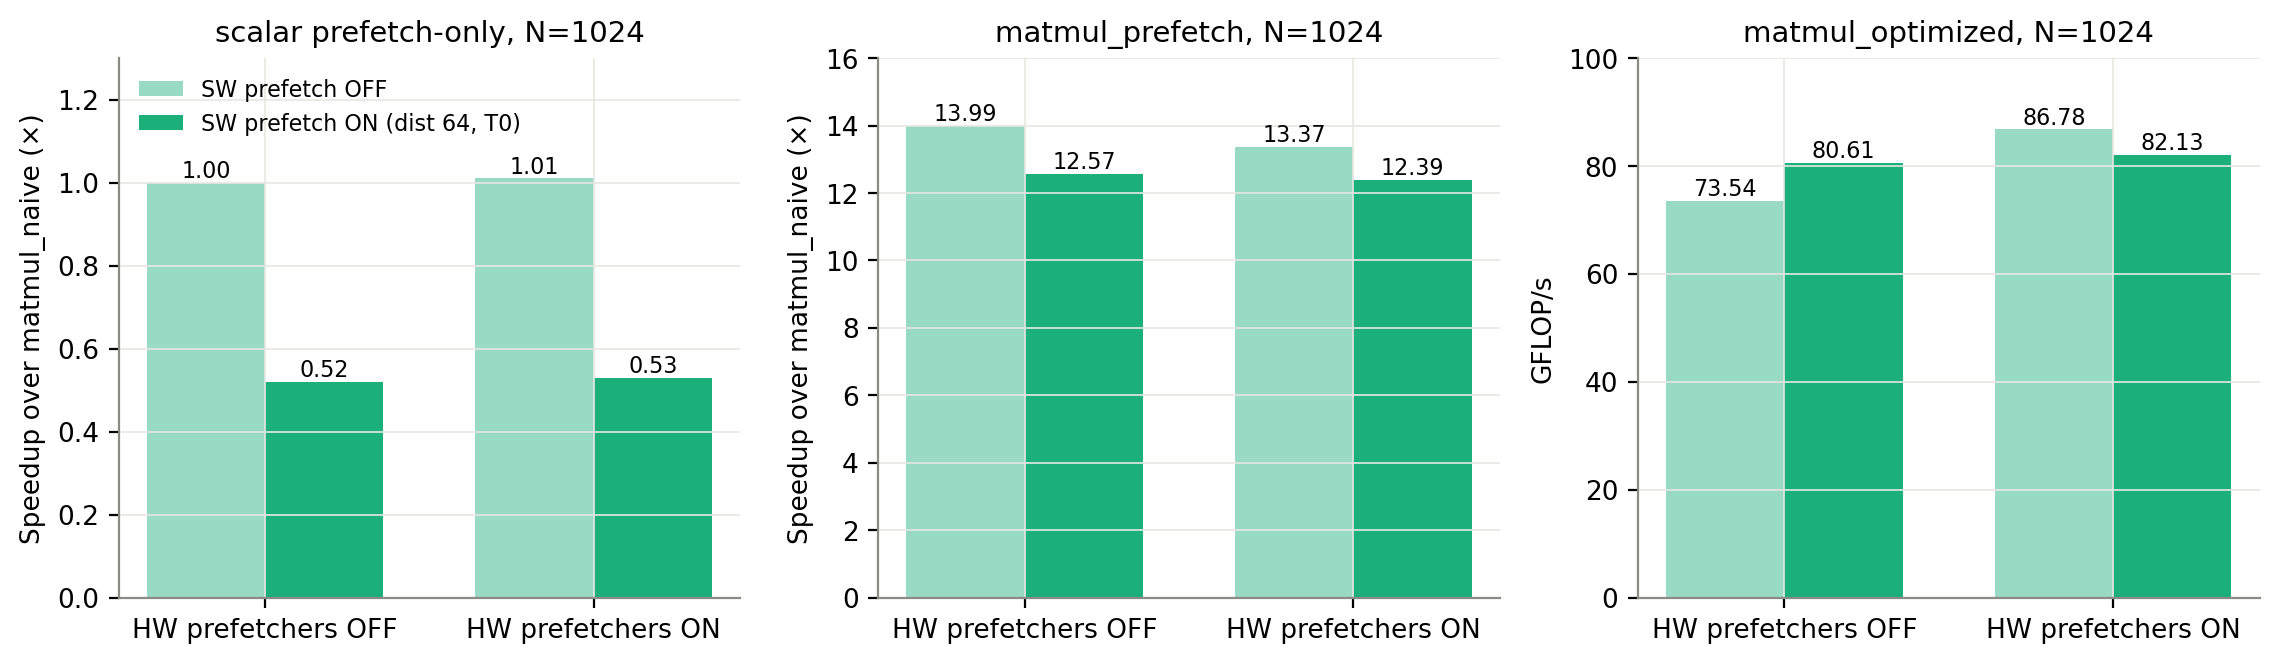
\includegraphics[width=\textwidth]{task2_hwpf.png}
\caption{Hardware prefetchers on/off crossed with software prefetch on/off for the three kernels.}
\label{fig:hwpf}
\end{figure}

\subsection{Answers}

\textbf{Q1.} Measured the way the assignment defines it ($t_{\text{without}}/t_{\text{with}}$), software prefetching stays below 1.0 at every size for every kernel on this machine: 0.50 to 0.60$\times$ for the scalar loop, 0.69 to 0.93$\times$ for the blocked SIMD kernel, and 0.94 to 0.98$\times$ for the combined kernel (Section~\ref{sec:2c}). The penalty shrinks as the matrix grows, from 0.69 at 128 to 0.88 to 0.93 at 1536 and 2048 for \texttt{matmul\_prefetch}. At small sizes everything is in L1 or L2 and the prefetch is pure overhead. At 2048 the working set is 48\,MB, more than L3, so there is real DRAM latency to hide, and the prefetch hides some of it: LLC misses halve, 2.35\,M to 1.07\,M (Table~\ref{tab:2a-miss-size}). Why it never reaches 1.0 is visible in Table~\ref{tab:hwpf}. With the hardware prefetchers on, the L2 streamer already covers this unit-stride pattern, so software prefetch removes L1 misses that were not on the critical path (348\,M to 48\,M) while its 671\,M extra instructions per $1024^3$ product eat issue bandwidth. Against naive, the prefetch stage is a flat 12 to 14$\times$ at all sizes, where the un-blocked SIMD kernel decays from 15$\times$ to 7$\times$. That flatness comes from the cache blocking, not from the prefetch.

\textbf{Q2.} By wall-clock the best distance is 0, i.e. no software prefetch, for all three kernels. Among the non-zero distances the blocked SIMD kernel does best at 64 floats (12.34$\times$, against 12.14 at 16 and 11.90 at 256), and the miss curve has the expected U shape. At 16 floats, one line ahead, L1 misses are lowest (41.6\,M) because the line has only just arrived when it is needed. 64 is nearly as good (48.3\,M) and gives the core more slack. At 256 floats, 1\,KB ahead, prefetched lines get evicted before use, misses climb back to 76.5\,M and LLC misses double. We therefore quote 64 floats (4 cache lines) as the best distance when prefetching is used: fastest among the non-zero distances and in the flat bottom of the miss curve. Distance does not change how many prefetches are issued (671\,M at every distance), only how far ahead they land.

\textbf{Q3.} T0. On \texttt{matmul\_prefetch} T0 gives 11.67$\times$ against 10.97 (T1), 10.91 (T2) and 11.01 (NTA), and the L1 miss counts show the hints doing what the manual says: T1 and T2 stop the line in L2/L3 and L1 misses triple (47\,M to 140\,M). NTA matches T0 on L1 misses but is the wrong hint here, because each $B$ panel is reused across all $M$ rows of $A$ and a non-temporal hint invites early eviction. The \texttt{sw\_prefetch\_access} counters confirm that the intended event fires for each hint (Table~\ref{tab:2a-params}). On the combined kernel the four hints land within 6\% of each other (Figure~\ref{fig:level}). The \texttt{JC}=32 panel is already in L2 before the inner loop starts, so the level the hint targets hardly matters; T0 and NTA are best at $N=2048$ (85.4 GFLOP/s).

Hardware prefetchers. Turning them off costs the blocked SIMD kernel only about 4\% (13.99 to 13.37$\times$ with SW prefetch off), because the panel blocking already keeps the working set in L2. The combined kernel is the interesting case. With the hardware prefetchers off, software prefetch turns from a 5.4\% loss into a 9.6\% gain (73.5 to 80.6 GFLOP/s). On this access pattern software and hardware prefetch substitute for each other: the hardware streamer handles unit-stride rows for free, and the software version only pays off when the hardware is absent.

\section{Task 2B: SIMD}

\begin{table}[H]
\centering\small
\caption{Table 2.1: instruction count (isolated single call) and execution time (harness median) by matrix size and SIMD width. 512-bit is not available on this CPU. Data: \texttt{task2b\_instr\_by\_width.txt}, \texttt{task2b\_simd\_width.txt}.}
\label{tab:21}
\begin{tabular}{l l rrr}
\toprule
& metric & $512^3$ & $1024^3$ & $2048^3$ \\
\midrule
\multirow{2}{*}{No SIMD (naive)} & instructions & 838,022,006 & 6,572,916,527 & 52,076,483,939 \\
 & time (ms) & 52.45 & 435.9 & 3588.0 \\
\midrule
\multirow{3}{*}{SIMD 128-bit (SSE4.2)} & instructions & 166,896,117 & 1,201,946,863 & 9,104,092,474 \\
 & time (ms) & 6.900 & 79.31 & 575.5 \\
 & speedup vs no SIMD & 7.55$\times$ & 5.78$\times$ & 6.23$\times$ \\
\midrule
\multirow{3}{*}{SIMD 256-bit (AVX2+FMA)} & instructions & 65,653,310 & 395,047,199 & 2,653,294,523 \\
 & time (ms) & 4.531 & 58.37 & 500.0 \\
 & speedup vs no SIMD & 11.58$\times$ & 7.47$\times$ & 7.18$\times$ \\
\midrule
SIMD 512-bit & & N/A & N/A & N/A \\
\midrule
\multirow{3}{*}{instruction reduction} & naive / 128 & 5.02$\times$ & 5.47$\times$ & 5.72$\times$ \\
 & naive / 256 & 12.76$\times$ & 16.64$\times$ & 19.63$\times$ \\
 & 128 / 256 & 2.54$\times$ & 3.04$\times$ & 3.43$\times$ \\
\bottomrule
\end{tabular}
\end{table}

\begin{figure}[H]
\centering
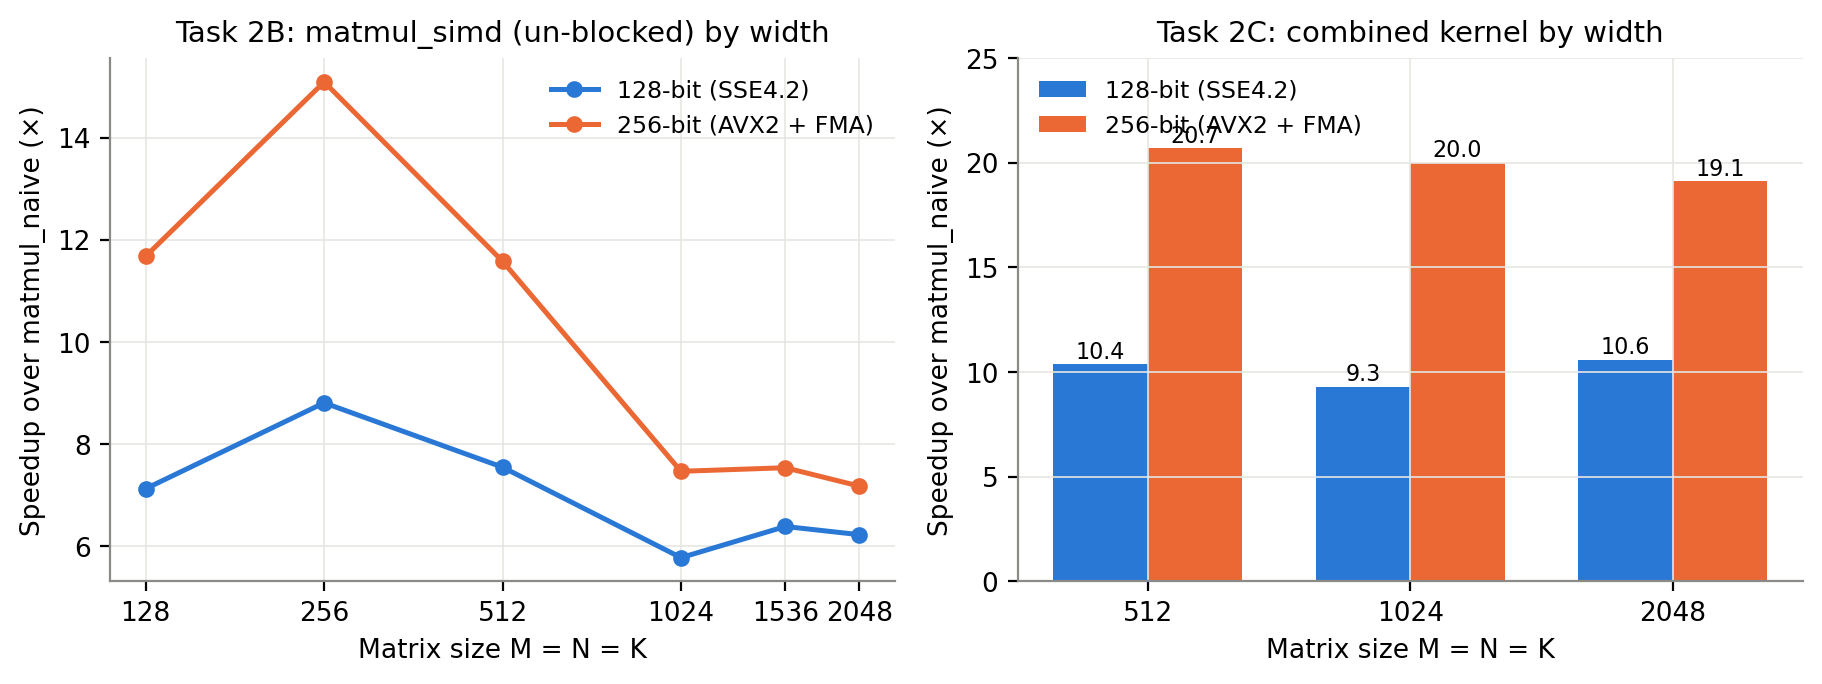
\includegraphics[width=\textwidth]{task2_simd_width.png}
\caption{Speedup over naive versus size by SIMD width. Left: the un-blocked \texttt{matmul\_simd} (Task 2B). Right: the combined kernel with an SSE port (Task 2C).}
\label{fig:width}
\end{figure}

\begin{table}[H]
\centering\small
\caption{\texttt{matmul\_simd} (256-bit) speedup over naive across sizes (\texttt{task2b\_sweep.txt}).}
\begin{tabular}{lrrrrrrrr}
\toprule
$M=N=K$ & 128 & 256 & 384 & 512 & 768 & 1024 & 1536 & 2048 \\
\midrule
GFLOP/s & 79.8 & 81.1 & 76.5 & 58.8 & 36.0 & 31.3 & 34.4 & 33.0 \\
speedup & 14.9$\times$ & 14.7$\times$ & 16.7$\times$ & 11.4$\times$ & 7.1$\times$ & 7.0$\times$ & 7.4$\times$ & 6.9$\times$ \\
\bottomrule
\end{tabular}
\end{table}

\subsection{Answers}

\textbf{Q1.} The 256-bit kernel cuts instructions 12.8 to 19.6$\times$: 8 lanes, times the FMA fusing the separate multiply and add, is about 16$\times$, and at larger $K$ the per-element loop overhead disappears as well. Time improves only 7 to 17$\times$, and the speedup has two regimes. Up to $384^3$, where all three matrices total at most 1.8\,MB and sit in L2, the kernel reaches 76 to 81 GFLOP/s and 15 to 17$\times$. From $512^3$ on it drops to about 7$\times$ and 31 to 36 GFLOP/s. The $1\times4$ kernel streams the whole of $B$ once per row of $A$ with no reuse, so once $B$ is bigger than L2 it is re-read from L3 or DRAM $M$ times and the kernel is bandwidth-bound; at $1024^3$ L1 misses go from 22\,M for naive to 198\,M for SIMD. The width comparison says the same thing from the other side. 256-bit beats 128-bit at every size, but the margin shrinks from 1.80$\times$ at 256 to 1.15$\times$ at 2048, because a wider vector unit does not help when the loads are the bottleneck. Two caveats on the 128-bit numbers. The SSE4.2 build has no FMA, so it issues separate \texttt{\_mm\_mul\_ps} and \texttt{\_mm\_add\_ps}, and the 128/256 instruction ratio is 2.5 to 3.4$\times$ rather than the 2$\times$ that width alone would give. And the $N=128$ points take less than a millisecond and are noisy.

\textbf{Q2.} 256-bit (AVX2 with FMA), at every size, with a peak of 16.7$\times$ at $384^3$. We could not test 512-bit. On the combined kernel, where cache blocking removes the bandwidth wall, the 256-bit margin is a steady 1.8 to 2.15$\times$ that does not depend on size (Figure~\ref{fig:width} right, Section~\ref{sec:2c}), which is what lane count predicts once the kernel is compute-bound.

{\sloppy Intrinsics. \texttt{\_mm256\_loadu\_ps}, because rows of llama.cpp tensors are not guaranteed to be 32\,B-aligned. \texttt{\_mm256\_fmadd\_ps}, one instruction and one rounding, which needs \texttt{-mfma}. \texttt{\_mm256\_setzero\_ps} for the accumulators. A horizontal-sum helper (\texttt{castps256\_ps128}, \texttt{extractf128}, \texttt{add\_ps}, two \texttt{hadd\_ps}, \texttt{cvtss\_f32}) that runs once per output element, outside the $K$ loop, since AVX2 has no single horizontal-add instruction. The 128-bit variant uses the \texttt{\_mm\_*} equivalents. We used single-precision \texttt{\_ps} intrinsics throughout because SGEMM is \texttt{float32}; the \texttt{\_pd} examples in the appendix would halve the lane count.\par}

\section{Task 2C: software prefetching + SIMD}
\label{sec:2c}

\subsection{Speedup versus size for every technique}

\begin{table}[H]
\centering\small
\caption{Speedup over naive of each stage, all four measured in the same harness run per size so they share a baseline. The $1536$ optimized value is the median of a 3-run recheck (\texttt{task2c\_recheck.txt}); the first-pass 14.86$\times$ was a scheduling outlier. Data: \texttt{task2c\_all\_stages\_vs\_size.txt}.}
\label{tab:2c-size}
\begin{tabular}{lrrrrrr}
\toprule
$M=N=K$ & 128 & 256 & 512 & 1024 & 1536 & 2048 \\
\midrule
SW prefetch only (scalar)           & 0.60$\times$ & 0.50$\times$ & 0.53$\times$ & 0.51$\times$ & -- & 0.51$\times$ \\
SIMD only (\texttt{matmul\_simd})   & 12.7$\times$ & 14.9$\times$ & 13.0$\times$ & 7.2$\times$ & 7.2$\times$ & 6.9$\times$ \\
SW prefetch + tiling + SIMD (\texttt{matmul\_prefetch}) & 14.4$\times$ & 12.2$\times$ & 12.6$\times$ & 12.6$\times$ & 12.4$\times$ & 12.0$\times$ \\
All combined (\texttt{matmul\_optimized}) & 13.8$\times$ & 18.3$\times$ & 19.9$\times$ & 19.1$\times$ & 18.5$\times$ & 18.2$\times$ \\
\quad GFLOP/s & 66.7 & 100.1 & 98.7 & 91.9 & 88.4 & 84.2 \\
\bottomrule
\end{tabular}
\end{table}

\begin{figure}[H]
\centering
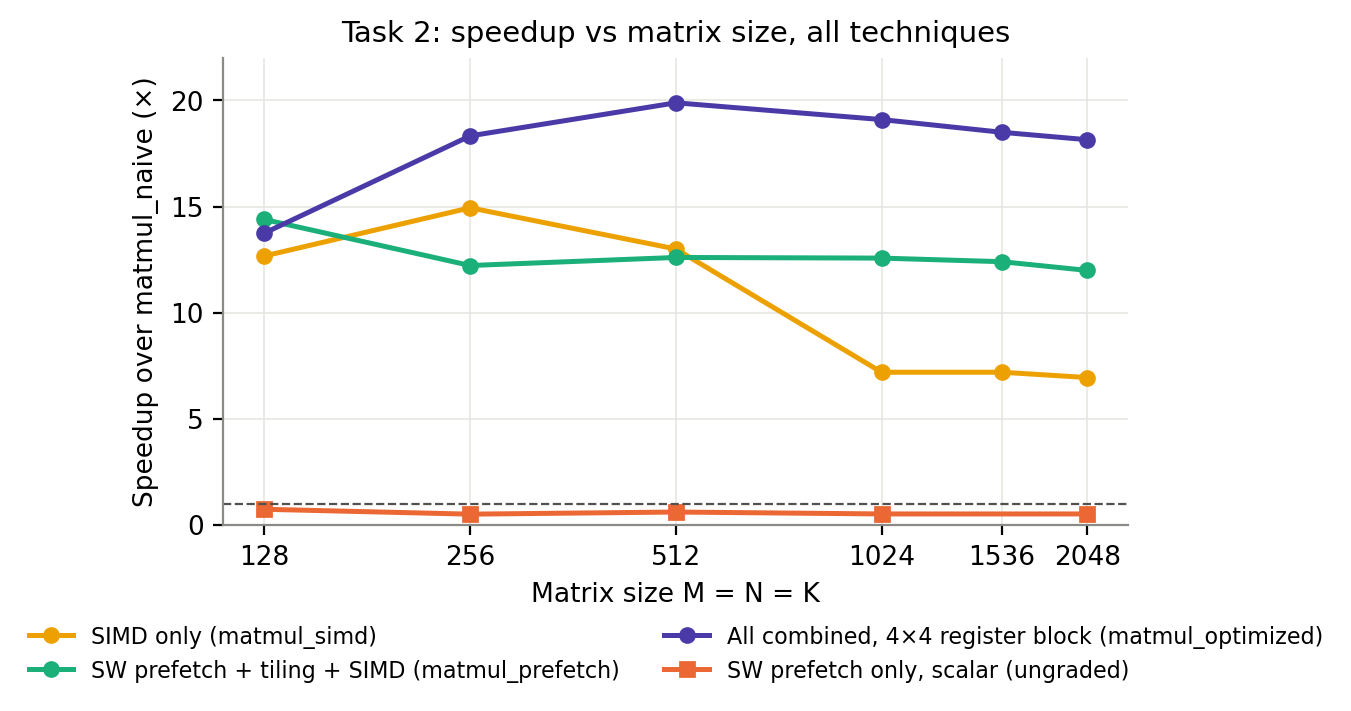
\includegraphics[width=0.78\textwidth]{task2_speedup_vs_size.png}
\caption{Final comparison: speedup over naive versus matrix size for software prefetching alone, SIMD alone, the prefetching stage built on SIMD and tiling, and the fully combined kernel.}
\label{fig:final}
\end{figure}

The three graded curves behave differently. SIMD alone falls from 15$\times$ to 7$\times$ once $B$ leaves L2. Adding cache blocking and prefetch to the same micro-kernel flattens the curve at about 12$\times$ but no higher, because the $1\times4$ kernel does only 4 FMAs per 5 vector loads and cannot use the locality it now has. The combined kernel is flat and high at 18 to 20$\times$. Its $4\times4$ register block does 16 FMAs per 8 loads, so the L2-resident panel is consumed at compute speed. At $1024^3$ the combined kernel (19.1$\times$) beats the best single stage (12.6$\times$) and the sum of the individual improvements; neither technique alone gets past about 15$\times$ at any size. On this Intel machine the harness scores \texttt{matmul\_optimized} at 18.2 to 19.9$\times$, which is 55/70 speedup points; the 25$\times$ top tier was out of reach.

\subsection{Repeating the 2A analyses on the combined kernel}

\begin{table}[H]
\centering\small
\caption{Combined kernel: prefetch distance and hint sweeps. $N=1024$ values are medians of 3 runs (\texttt{task2c\_recheck.txt}); 512 and 2048 from \texttt{task2c\_width\_and\_extra\_sizes.txt}. GFLOP/s is quoted because the naive baseline drifted between 418 and 470\,ms across harness invocations, which perturbs the speedup column more than the kernel itself.}
\label{tab:2c-params}
\begin{tabular}{l rrrrrr}
\toprule
distance (floats) & 0 & 16 & 32 & 64 & 128 & 256 \\
\midrule
$N=512$ GFLOP/s   & \textbf{103.0} & 101.0 & -- & 100.9 & -- & 96.3 \\
$N=1024$ GFLOP/s  & \textbf{90.3} & 84.9 & 84.6 & 84.8 & 83.9 & 84.2 \\
$N=2048$ GFLOP/s  & \textbf{89.7} & 85.1 & -- & 85.1 & -- & 85.7 \\
\midrule
hint (distance 64) & T0 & T1 & T2 & NTA & & \\
\midrule
$N=1024$ GFLOP/s  & 80.7 & 81.9 & 78.1 & 82.9 & & \\
$N=2048$ GFLOP/s  & 85.4 & 82.9 & 82.8 & 85.4 & & \\
\bottomrule
\end{tabular}
\end{table}

\begin{table}[H]
\centering\small
\caption{Combined kernel: cache misses and throughput without and with software prefetch (distance 64, T0). \texttt{task2c\_cachemiss.txt}; $N=2048$ throughput from the 3-run recheck.}
\setlength{\tabcolsep}{4pt}\footnotesize
\begin{tabular}{l rr rr rr rr}
\toprule
& \multicolumn{2}{c}{L1-D misses} & \multicolumn{2}{c}{L2 misses} & \multicolumn{2}{c}{LLC misses} & \multicolumn{2}{c}{GFLOP/s} \\
\cmidrule(lr){2-3}\cmidrule(lr){4-5}\cmidrule(lr){6-7}\cmidrule(lr){8-9}
$N$ & without & with & without & with & without & with & without & with \\
\midrule
1024 & 57.2\,M & 44.8\,M & 424\,M & 424\,M & 32.6\,K & 24.5\,K & 87.0 & 83.5 \\
2048 & 635\,M & 440\,M & 3408\,M & 3403\,M & 1.36\,M & 0.78\,M & 82.7 & 78.2 \\
\bottomrule
\end{tabular}
\end{table}

Speedup versus size and parameters (2A questions 1 to 3 on the combined kernel). The assignment-defined speedup of software prefetch on the combined kernel is 0.98$\times$ at 512, 0.94$\times$ at 1024 and 0.95$\times$ at 2048, a steady 4 to 6\% loss that again shrinks a little with size. The best distance is 0 at every size, and the non-zero distances all sit within 1 to 2\% of each other; the combined kernel does not care about distance because the panel is already in L2. The best hints are T0 and NTA (85.4 GFLOP/s at 2048), with T1 and T2 about 3\% behind. Prefetching does work at the cache level, with 22 to 31\% fewer L1 misses and 25 to 43\% fewer LLC misses. L2 misses do not change, since prefetch changes when a line arrives and not how many lines the working set needs. But the misses it removes were already hidden behind the 16-FMA inner loop. That is why the graded \texttt{matmul\_optimized.cpp} ships with \texttt{PF\_D}=0: the prefetch code is there and tunable, and the measurements said to leave it off.

Hardware prefetchers (2A question 5). Here the combined kernel behaves differently from the earlier ones (Table~\ref{tab:hwpf}, Figure~\ref{fig:hwpf}). With hardware prefetching disabled, software prefetch is a 9.6\% gain (73.5 to 80.6 GFLOP/s); with it enabled, the same code is a 5.4\% loss. The combined kernel is fast enough that memory latency is a visible share of its runtime, so once the hardware streamer is gone the software version has something to do. Software and hardware prefetch substitute for each other on this unit-stride pattern, and the graded default (\texttt{PF\_D}=0) is the right one for a machine with its hardware prefetchers on, which is the normal case.

\begin{table}[H]
\centering\small
\caption{Instruction count and time, isolated single call (\texttt{task2c\_instr.txt}).}
\setlength{\tabcolsep}{3.5pt}\scriptsize
\begin{tabular}{l rrr rr}
\toprule
$N$ & naive instr. & SIMD instr. & combined instr. & naive / combined & SIMD / combined \\
\midrule
1024 & 6,572,879,294 & 395,350,711 & 352,332,734 & 18.7$\times$ & 1.12$\times$ \\
2048 & 52,084,965,519 & 2,656,656,781 & 2,313,442,978 & 22.5$\times$ & 1.15$\times$ \\
\midrule
wall-clock 1024 (s) & 0.466 & 0.0757 & 0.0376 & 12.4$\times$ & 2.01$\times$ \\
wall-clock 2048 (s) & 3.935 & 0.639 & 0.245 & 16.1$\times$ & 2.61$\times$ \\
\bottomrule
\end{tabular}
\end{table}

Instruction count (2B question 1 on the combined kernel). The combined kernel executes only 12 to 15\% fewer instructions than SIMD alone, the saving coming from the $4\times4$ block's fewer loads and horizontal sums, yet it runs 2.0 to 2.6$\times$ faster. Its advantage is instructions per cycle, not instruction count. Cache blocking lets the same instruction stream retire about twice as fast because the operands come from L2 instead of DRAM. SIMD cuts the count 16 to 20$\times$; tiling and register blocking raise the rate.

SIMD width (2B question 2 on the combined kernel). With a full SSE port of the $4\times4$, \texttt{JC}=32 kernel the comparison is like for like: 10.4 / 9.3 / 10.6$\times$ for 128-bit against 20.7 / 20.0 / 19.1$\times$ for 256-bit at 512 / 1024 / 2048, a ratio of 2.0 / 2.15 / 1.8. Unlike the un-blocked kernel, this ratio does not shrink with size, because both widths are now compute-bound. Part of it is FMA fusion, which SSE4.2 lacks, so lane width alone accounts for somewhat less than 2$\times$. The 128-bit port is correct on the ragged shapes $255\times257\times129$, $1\times129\times130$ and $3\times3\times3$.

\subsection{Inside llama.cpp}

\texttt{make llama-demo} clones llama.cpp \texttt{b5731}, builds a stock \texttt{llama-cli}, injects \texttt{matmul\_optimized} into ggml's single-threaded F32 \texttt{mul\_mat} path and rebuilds, then runs \texttt{stories260K.gguf} (F32, 1.2\,MB) on both builds with one thread, a fixed seed and the same prompt. Both checks pass:
\begin{quote}\small\ttfamily
[ok] student matmul\_optimized was actually used by ggml\\
{[ok]} student output matches stock output token-for-token (kernel is correct)
\end{quote}
This runs the kernel under ggml's own tensor strides (non-contiguous \texttt{lda}, \texttt{ldb}, \texttt{ldc}) and on the $M=1$ generation path, neither of which the microbenchmark covers, so it is the correctness result that matters.

Throughput on this model is at parity within noise, and we do not claim a win or a loss. Over five paired runs the student/native ratio was 0.94 to 1.21 for prompt evaluation (median 1.00) and 0.96 to 1.06 for generation (median 1.04), while the native binary by itself varied 1.44$\times$ between runs (6.9\,k to 9.9\,k tokens/s). The whole inference takes about 6\,ms, prompt evaluation is timed over five tokens (0.3\,ms), the model's matrices fit in L1 so cache blocking has nothing to do, and generation runs at $M=1$, where the kernel takes its vectorised tail rather than the $4\times4$ path. Performance claims for the kernel rest on the microbenchmark, where the matrices are big enough for blocking to matter.

\section{Summary}

Software prefetching (2A) on a scalar loop halves throughput, because a per-element prefetch doubles an issue-bound loop. Issued once per vector on the blocked SIMD kernel it removes 7$\times$ the L1 misses and half the LLC misses at 2048, with the expected U-shaped miss curve (best 16 to 64 floats ahead) and hint behaviour (T0 best, T1 and T2 triple the L1 misses), yet it still costs 7 to 17\% in time because the hardware streamer already covers the pattern. SIMD (2B) cuts instructions 12.8 to 19.6$\times$ and gives 15 to 17$\times$ while the data fits in L2, decaying to 7$\times$ beyond that; 256-bit beats 128-bit at every size. Combining register blocking, SIMD, cache tiling and optional prefetch (2C) gives a flat 18 to 20$\times$ at 84 to 100 GFLOP/s across all sizes, a like-for-like 2$\times$ from 256-bit over 128-bit, and twice the IPC of SIMD alone on 12\% fewer instructions. Software prefetch only becomes a gain (9.6\%) when the hardware prefetchers are disabled, so the shipped kernel keeps it off. Inside llama.cpp the same kernel reproduces the native matmul's output token for token.

\end{document}
